\documentclass[crop,tikz]{standalone}

\begin{document}
  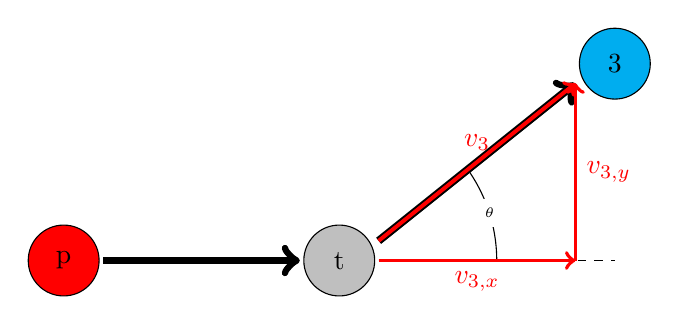
\begin{tikzpicture}
    \node[circle, draw, fill=red, minimum size = 0.9cm] (c) at (-3.5,0){p}; 
    \draw [-to, line width=1mm] (-3,0) -- (-0.5,0);
    \node[circle, draw, fill=lightgray, minimum size = 0.9cm] (c) at (0,0){t}; 
    \node[circle, draw, fill=cyan, minimum size = 0.9cm] (c) at (3.5, 2.5){$3$}; 
    \draw [-to, line width=1mm] (0.5,0.25) -- (3,2.25);
    \draw [dashed] (0.5,0) -- (3.5,0);
    \draw (2,0) arc [start angle=0, end angle=35, x radius=2cm, y radius =2cm] node[midway,fill=white] {{\tiny $\theta$}};
    \draw [-to, line width=0.5mm,red] (0.5,0) -- (3,0) node[midway,below] {$v_{3,x}$};
    \draw [-to, line width=0.5mm,red] (3,0) -- (3,2.25) node[midway,right] {$v_{3,y}$};
    \draw [-to, line width=0.5mm,red] (0.5,0.25) -- (3,2.25) node[midway,above] {$v_{3}$};
  \end{tikzpicture}
\end{document}